%
% chapter3.tex
%

\chapter{Design}
\label{cha:design}
The following chapter discusses the design of the socket IPC for Simplefail2ban.
While reasoning the choice of unix domain sockets, advantages and disadvantages are presented.

\section{Reasoning for Unix Domain Sockets}
In order to make an informed decision on which IPC type is suited best for an IPC method, requirements need to be specified.
Since the task at hand is to defend against DoS like attacks on the host system, the following aspects are considered\cite{raatschen:ipc}:

\begin{itemize}
    \item \textbf{Low latency} \\
        Responding quickly to incoming threats is key to successfully block incoming attacks.
        A quick transfer of data to the IPS facilitates faster banning of malicious attackers, before they can overwhelm the system.
        In general, low overhead is required to achieve these goals.
    \item \textbf{High bandwidth} \\
        Considering that the host system is bombarded with millions of packets each second during an ongoing DoS attack, high bandwidth is crucial.
        To avoid bottlenecks between the writer and the IPS, large amounts of data need to be transmissible at once instead of requiring separate transmissions.
    \item \textbf{Reliability} \\
        Ensuring that no crucial log messages are lost due to unreliability is desirable.
        Repeatedly missing information about malicious clients delays the response time of the IPS, risking uptime of the system and its services.
    \item \textbf{Scalability} \\
        Log messages can come from a multitude of sources and contain a variety of information.
        Multiple applications should be able to submit log messages to the IPS at once and retain the possibility of providing it to other applications.
        Therefore, the option to have both multiple readers and writers needs to be present.
        Furthermore, while not necessary for the development of a host-based IPS, the option to scale beyond the local filesystem is interesting.
    \item \textbf{Portability} \\
        Developing an IPS requires it to actually be usable with already existing applications.
        Whereas this thesis is not intended to be more than a demonstration of a proof of concept, potential future development still requires some flexibility.
        A well defined API that can realistically be integrated into any real application without the need for specific hard- and software is a bare minimum.
\end{itemize}

Initially, the decision by Paul Raatschen to use shared memory as the IPC method used in Simplefail2ban was mainly based on the fact that the kernel was not involved in any read or write operations\cite{raatschen:ipc}.
Yet, no other IPC method was implemented.
To ensure that the shared memory approach is the most viable, an alternative needed to be chosen to be measured against.

The choice fell on unix domain sockets, due to the already existing read and write API and its support in the Posix standard on all UNIX systems since at least 2007\cite{posix}.
Additionally, the utilization of sockets provided a great deal of flexibility during usage of the IPC which will be discussed in the next section.

\section{Design and abstractions}
\label{sec:Design_and_abstractions}
During the design process of the socket architecture it was decided that supporting attachment of multiple readers was essential, as already discussed in section \ref{sec:Reasoning for Unix Domain Sockets}.
Each reader should receive all log messages sent by any writers.
These restrictions led to the design illustrated in \ref{fig:socket:architecture}. TODO: Update this graphic + Dataflow

\begin{figure}[h!]
    \centerline{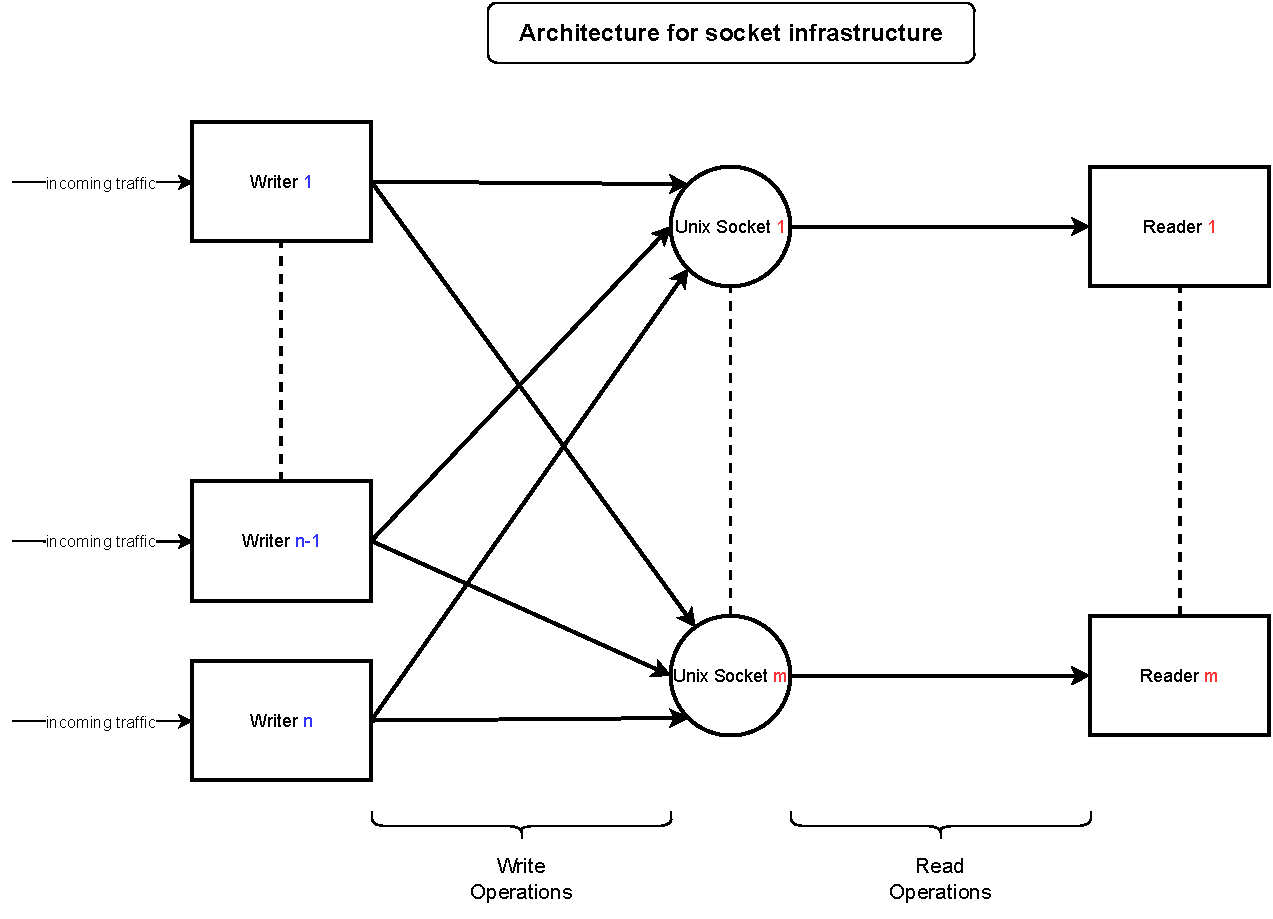
\includegraphics[width=1.2\textwidth]{images/SocketArchitecture.pdf}}
    \caption[General design of socket architecture]{
        Architecture for a n-reader and m-writers scenario using UNIX domain sockets.}
	\label{fig:socket:architecture}
\end{figure}

The figure displays the general data flow using the socket IPC.
Each reader application creates its own UNIX domain socket.
Sockets are bound to a filesystem pathname.
Readers can receive data from their own socket without having to compete or synchronize with other readers for data thanks to the one-to-one mapping between socket and reader.
Meanwhile, writers can also independently write data into sockets without having to communicate with other writer processes.
In order to guarantee that readers receive all data being sent via the socket IPC architecture, writers need to periodically recheck for newly opened sockets and always send their data to all available sockets.
This results in the writers having a significant portion of the overhead, needing to resend identical data multiple times.
Minimizing overhead on the reader side is important to maximize the limited computational time crucial services, such as the IPS Simplefail2ban, need to process incoming log messages.

To preserve the integrity of log messages, the unix domain socket needs to retain message boundaries, ruling out the SOCK\_STREAM unix domain socket presented in section \ref{Unix Domain Sockets}.
Without the absolute guarantee of reliable behavior in regard to reordering of messages - which is only present in most UNIX implementation but not all\cite{man:unixsockets} - SOCK\_DGRAM is unappealing as well.
Therefore, the socket type choice falls on SOCK\_SEQPACKET, a connection-oriented option that retains message-boundaries and sequence.